\section{非仿射随机波动率模型：真正需要数值积分的部分}\label{sec:nonaffine}
\subsection{为什么再增加一个随机变量？}
GBM 假设波动率 $\sigma$ 不变。为了表达波动强度随时间随机变化，题目引入因子 $Y_t$，再用函数 $g$ 把它变成实际波动率。
原题直接给出对数价格 $X_t=\log S_t$ 的系统：
\begin{align}
 dX_t&=\left(\mu-\frac12g(Y_t)^2\right)dt+g(Y_t)\,dW_t^{(1)},\label{eq:na-x}\\
 dY_t&=\kappa(\theta-Y_t)dt+\xi\sqrt{1+Y_t^2}\,dW_t^{(2)},\label{eq:na-y}\\
 g(y)&=\sigma_{\min}+\frac{\sigma_{\max}-\sigma_{\min}}{1+e^{-y}}.\label{eq:na-logistic}
\end{align}
这里 $Y_t$ 是\emph{波动率因子}，不是波动率本身。
它可以为负；只要将 $Y_t$ 代入 $g$，就得到正的实际波动率。
初值和参数见表~\ref{tab:na-parameters}。

\begin{table}[htbp]\centering\small
\caption{原题规定的非仿射基准参数及其作用。}\label{tab:na-parameters}
\begin{tabularx}{\textwidth}{llY}\toprule
参数 & 数值 & 含义\\\midrule
$S_0,X_0$ & $100,\log100$ & 初始价格与对数价格\\
$Y_0$ & $0$ & 初始波动因子；对应 $g(0)=0.30$\\
$\mu$ & $0.05$ & 价格的相对漂移率\\
$\kappa$ & $2$ & 因子向中心回复的强度\\
$\theta$ & $-0.2$ & 因子漂移项的回复中心\\
$\xi$ & $0.6$ & 波动因子的随机变化强度\\
$\rho$ & $-0.7$ & 两个布朗驱动在同一时段的增量相关系数\\
$\sigma_{\min},\sigma_{\max}$ & $0.10,0.50$ & 资产瞬时波动率的上下界\\
$T,K$ & $1,100$ & 终止时刻、收益函数的执行价\\\bottomrule
\end{tabularx}
\end{table}

若 $Y_t>\theta$，漂移 $\kappa(\theta-Y_t)$ 为负；若 $Y_t<\theta$，漂移为正。
这称为均值回复。它不是保证每一步都向 $\theta$ 移动，因为随机项可以盖过漂移。
在可积条件下，取期望还能得到 $m_Y'(t)=\kappa(\theta-m_Y(t))$，因而
\begin{equation}\label{eq:na-y-mean}
 \E Y_t=\theta+(Y_0-\theta)e^{-\kappa t}.
\end{equation}
这只是因子的均值，不能把它代入 $g$ 当成平均波动率：通常 $\E[g(Y_t)]\ne g(\E Y_t)$。

Logistic 函数随 $y$ 增大而增大，且
\begin{equation}\label{eq:na-g-bounds}
 0.1<g(y)<0.5,\qquad
 0<g'(y)=0.4\frac{e^{-y}}{(1+e^{-y})^2}\le0.1.
\end{equation}
因子扩散幅度 $0.6\sqrt{1+y^2}$ 在 $y=0$ 也不为零，离零越远越大。
但资产波动率仍由 $g$ 限制在固定区间内；“因子可能较大”不表示“资产波动率无限大”。

\begin{figure}[htbp]\centering
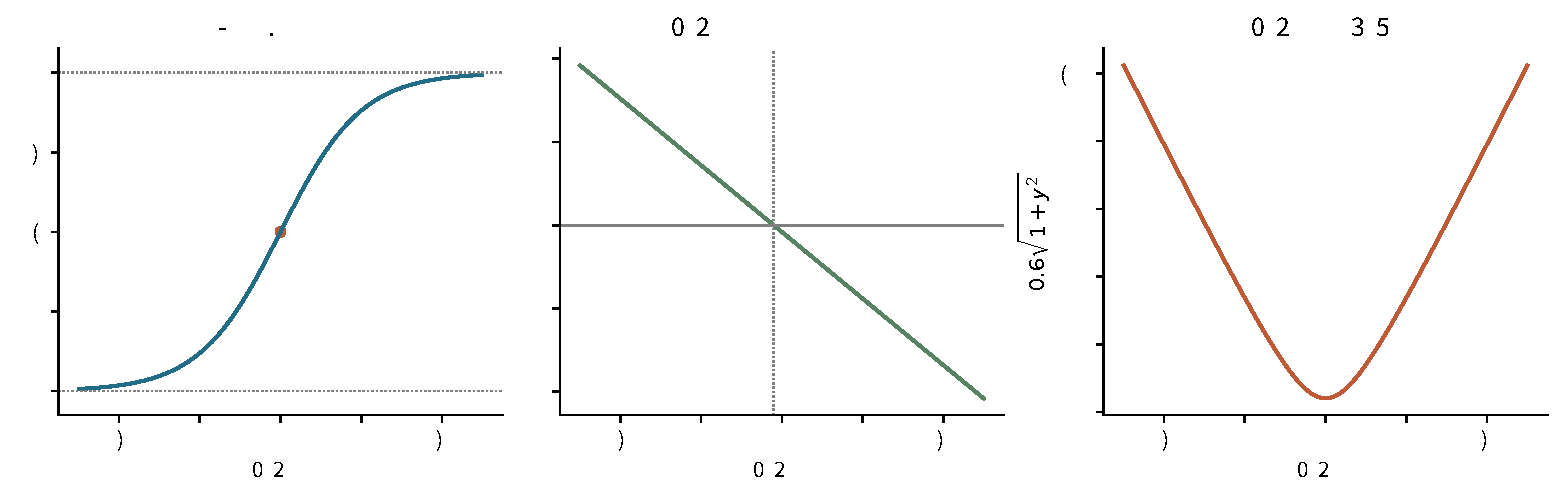
\includegraphics[width=\textwidth]{assets/model_functions.pdf}
\caption{模型函数的含义。左图为有界波动率；中图的正负号决定回复方向；右图是因子的随机扩散幅度。这些是题设函数曲线，不是模拟得到的经验规律。}\label{fig:na-functions}
\end{figure}
图~\ref{fig:na-functions} 将三个容易混淆的函数并列展示：资产的波动率是左图，因子的漂移与扩散分别是中图和右图。

\subsection{相关的布朗运动怎样由独立正态数生成？}
两种随机冲击可以相关，但它们不是同一个冲击。
从相互独立的 $Z_1,Z_2\sim N(0,1)$ 出发，设置
\begin{equation}\label{eq:na-correlated}
 \Delta W^{(1)}=\sqrt h Z_1,\qquad
 \Delta W^{(2)}=\sqrt h\bigl(\rho Z_1+\sqrt{1-\rho^2}Z_2\bigr).
\end{equation}
逐项计算就能验证：
\begin{align}
 \Var(\Delta W^{(2)})&=h\{\rho^2+(1-\rho^2)\}=h,\label{eq:na-driver-var}\\
 \Cov(\Delta W^{(1)},\Delta W^{(2)})&=h\rho,\qquad
 \operatorname{Corr}(\Delta W^{(1)},\Delta W^{(2)})=\rho.\label{eq:na-driver-cov}
\end{align}
原题记号 $d\langle W^{(1)},W^{(2)}\rangle_t=\rho\,dt$ 描述两个驱动的二次协变差：把前面的增量平方和改为同一时段两个增量的乘积和，其极限为 $\rho t$。
在 Itô 运算中，它对应 $dW^{(1)}dW^{(2)}=\rho\,dt$ 的记账规则。
不同时间段仍用新的独立正态对。

$\rho=-0.7$ 的直觉是：驱动价格的冲击偏负时，驱动因子的冲击倾向偏正，于是波动率倾向升高。
这是即时随机冲击的倾向，不是每一条路径的确定规律。
它也不是 $S_T$ 和 $Y_T$ 两个终值的相关系数；后者受整个非线性系统共同影响。
遗漏 $\sqrt{1-\rho^2}$、直接使用 $\rho Z_1+Z_2$，会把第二个增量方差变成 $(1+\rho^2)h$，模拟的是错误模型。

\subsection{“非仿射”具体指什么？}
“仿射”指常数加状态的一次函数。
在仿射扩散模型中，关键通常是漂移和\emph{瞬时协方差矩阵}对状态具有仿射结构，而不只是扩散系数表面上是否有平方根。
因此不能说“出现平方根就一定非仿射”。
本模型的瞬时协方差矩阵如下；在很短的时间 $h$ 内，$(\Delta X,\Delta Y)$ 的条件协方差矩阵近似为它乘以 $h$：
\begin{equation}\label{eq:na-cov-matrix}
 \begin{pmatrix}
  g(y)^2 & \rho\xi g(y)\sqrt{1+y^2}\\
  \rho\xi g(y)\sqrt{1+y^2} & \xi^2(1+y^2)
 \end{pmatrix}.
\end{equation}
其中 $g(y)^2$ 和 $1+y^2$ 不是状态的一次函数，$X$ 的漂移也含 $g(y)^2$，所以不具备该结构。
这个名称主要帮助理解模型类别；写出 EM 并不需要先掌握整个仿射过程理论。

\subsection{对两个状态同步使用左端 EM}
一步开始时已知 $X_n,Y_n$，先计算 $g_n=g(Y_n)$，再使用同一时段的两维增量：
\begin{align}
 X_{n+1}&=X_n+(\mu-g_n^2/2)h+g_n\Delta W_n^{(1)},\label{eq:na-em-x}\\
 Y_{n+1}&=Y_n+\kappa(\theta-Y_n)h+\xi\sqrt{1+Y_n^2}\Delta W_n^{(2)},\label{eq:na-em-y}\\
 S_{n+1}&=e^{X_{n+1}}.\label{eq:na-em-s}
\end{align}
两条式子的系数都使用\emph{旧的} $Y_n$。
若先更新 $Y$，再将 $Y_{n+1}$ 放进 $X$ 的系数，同一步的新噪声就进入了扩散系数，这已改变离散方法。
尤其当两个驱动相关时，这种修改不只是代码顺序的无害变化。

做一次手算：取 $h=0.01$、$X_n=\log100$、$Y_n=0$，这一步 $Z_1=1$、$Z_2=0$。
由式~\eqref{eq:na-correlated} 得 $\Delta W^{(1)}=0.1$、$\Delta W^{(2)}=-0.07$；此时 $g_n=0.3$。
所以
\begin{equation}\label{eq:na-hand-step}
 \Delta X=0.005(0.01)+0.3(0.1)=0.03005,\qquad
 Y_{n+1}=0+2(-0.2)(0.01)+0.6(-0.07)=-0.046.
\end{equation}
价格为 $100e^{0.03005}\approx103.0506$。
新的 $Y=-0.046$ 会影响\emph{下一步}的波动率，不回头改变这一步已经使用的 $0.3$。

在实数运算中，$e^X>0$ 自动成立。在浮点运算中，极端大的 $X$ 可能上溢、极端小的 $X$ 可能下溢到零。
现有程序不仅检查终值，还追踪所有网格步的 $X,Y$ 极值与有限性，确认指数处于可表示的正有限范围。
这比仅看到最终数组没有 NaN 更有说服力。

\subsection{为什么不照搬一维 Milstein？}
将相关驱动写成两个独立布朗运动 $B^{(1)},B^{(2)}$，令 $a(y)=\xi\sqrt{1+y^2}$、$c=\sqrt{1-\rho^2}$，对应扩散向量是
\begin{equation}\label{eq:na-diffusion-columns}
 b_1(x,y)=\binom{g(y)}{\rho a(y)},\qquad b_2(x,y)=\binom{0}{ca(y)}.
\end{equation}
二维随机 Taylor 展开通常还会出现 $\int(B^{(1)}_s-B^{(1)}_{t_n})\,dB_s^{(2)}$ 等交叉迭代积分。
一维时，同一个噪声的迭代积分可化为 $(\Delta W^2-h)/2$；两个不同噪声的交叉信息一般不能仅由两个终点增量恢复。
本模型两种噪声的作用也不满足简化交叉项所需的交换条件。
这里 $Db_j$ 是向量函数 $b_j$ 的一阶偏导组成的矩阵，$(Db_j)b_k$ 衡量沿另一噪声方向移动时 $b_j$ 怎样变化：
\begin{equation}\label{eq:na-noncommute}
 (Db_2)b_1-(Db_1)b_2=\binom{-ca(y)g'(y)}0\ne0.
\end{equation}
初读时只需要记住：把标量修正项分别粘到两个方程上，并不能得到这个系统的强一阶方法。
原题明确要求本模型使用 EM；现有实现遵循这个要求。

\subsection{从理论上为什么预期出现半阶？进阶说明}
函数 $g$ 有界且导数有界，而
$\frac{d}{dy}\sqrt{1+y^2}=y/\sqrt{1+y^2}$ 的绝对值不超过 1。
因此 $(X,Y)$ 系统的漂移和扩散对状态全局 Lipschitz，并满足线性增长界。
标准 EM 理论在这里给出状态的终值均方根误差 $O(\sqrt h)$。

从 $X$ 转回 $S=e^X$ 需要多一步，因为指数函数不是全局 Lipschitz。
利用
\begin{equation}\label{eq:na-exp-error}
 |e^x-e^y|\le(e^x+e^y)|x-y|,
\end{equation}
再应用 Cauchy--Schwarz 不等式：
\begin{equation}\label{eq:na-strong-bound}
 \E|S_T^{(h)}-S_T|
 \le \sqrt{\E[(S_T^{(h)}+S_T)^2]}\,
       \sqrt{\E|X_T^{(h)}-X_T|^2}.
\end{equation}
有界的 $g$ 使第一因子对步长一致有界。例如离散方案满足
$\E[(S_{n+1})^2\mid\mathcal F_{t_n}]=S_n^2e^{2\mu h+g_n^2h}$，
故 $\E[S_N^2]\le S_0^2e^{(2\mu+\sigma_{\max}^2)T}$；连续模型也有同样形式的二阶矩上界。
于是价格终值的 $L^1$ 强误差有 $O(\sqrt h)$ 上界。
这说明半阶有理论依据，但\emph{现有图中直接测量的量}仍然是两个数值解之间的差，不能改称真误差。

\section{没有精确解时，怎样判断数值结果可信？}\label{sec:reference}
\subsection{三个参考网格也必须共享同一套噪声}
现有非仿射实验有 $100000$ 条路径。
粗网格步数为 $8,16,32,64,128,256$，参考网格步数为 $2048,4096,8192$。
程序先在 $8192$ 步生成两维相关增量，再通过相邻求和生成\emph{所有}其他网格。
三个参考仍是 EM，只是步长更小；较细并不意味着数学上精确。

设未知真解终值为 $S_T^\star$，粗解为 $S_T^{(h)}$，参考为 $S_T^{(r)}$。
三角不等式及反三角不等式给出
\begin{equation}\label{eq:ref-triangle}
 \left|\E|S_T^{(h)}-S_T^\star|-\E|S_T^{(h)}-S_T^{(r)}|\right|
 \le\E|S_T^{(r)}-S_T^\star|.
\end{equation}
右侧才是参考真误差，却是未知的。
将 $r$ 加密到 $r/2$，能观察的是 $\E|S_T^{(r)}-S_T^{(r/2)}|$。
它是参考敏感度的证据，不是式~\eqref{eq:ref-triangle} 右侧的已知上界。
如果两个参考共享相似的离散误差，它们可以非常接近而仍共同偏离真解。

\subsection{现有的 10\% 筛查应怎样理解？}
最后两层参考之间的平均绝对差为 $0.04015705$。
现有报告将它除以各粗网格相对最细参考的强差，作为一个实践性比例：
\begin{equation}\label{eq:ref-screen}
 R_h=\frac{\widehat\E|S_T^{(1/4096)}-S_T^{(1/8192)}|}
 {\widehat\E|S_T^{(h)}-S_T^{(1/8192)}|}.
\end{equation}
在预先指定的主拟合窗口 $N=8,16,32,64$，该比值约为 $3.20\%,4.46\%,6.29\%,8.89\%$，都低于 10\%。
到了 $N=128,256$，则约为 $12.61\%,17.99\%$，说明更细的粗网格相对更加受参考分辨率影响。

10\% 不是随机分析定理给出的万能阈值，而是原实验使用的敏感度标准。
正确结论是“主窗口对最后一次参考加密的变化相对不太敏感”，不是“参考真误差已被严格证明低于粗误差的 10\%”。
两个连续加密差从 $0.05679005$ 降到 $0.04015705$，比例约为 $0.7071$，与半阶缩放相容。
这仍然是数值证据；没有额外渐近假设或误差界，不能将其中一个差直接变成严格误差证书。

\subsection{为什么本模型不能再只检查价格均值？}
对 $S=e^X$ 应用 Itô 公式：
\begin{equation}\label{eq:ref-price-sde}
 dS_t=S_t\left[(\mu-g(Y_t)^2/2)dt+g(Y_t)dW_t^{(1)}\right]
       +\frac12S_tg(Y_t)^2dt
 =\mu S_tdt+g(Y_t)S_t\,dW_t^{(1)}.
\end{equation}
有界波动率提供足够的可积性，使随机积分均值为零；因此 $\E S_T=S_0e^{\mu T}$。
严格地说，可以先由有界 $g$ 得到有限二阶矩，再对积分方程取期望，解线性积分方程。

更特别的是，log-EM 也保留这个均值。
在第 $n$ 步开始时，$S_n$ 和 $g_n=g(Y_n)$ 都已知。
下一步 $\Delta W_n^{(1)}$ 与过去信息独立，条件下服从 $N(0,h)$，所以
\begin{equation}\label{eq:ref-discrete-mean}
\begin{aligned}
 \E[S_{n+1}\mid\mathcal F_{t_n}]
 &=S_ne^{(\mu-g_n^2/2)h}\E[e^{g_n\Delta W_n^{(1)}}\mid\mathcal F_{t_n}]\\
 &=S_ne^{(\mu-g_n^2/2)h}e^{g_n^2h/2}=e^{\mu h}S_n.
\end{aligned}
\end{equation}
反复取期望，所有步长都得到 $\E S_N=S_0e^{\mu T}$。
两个布朗驱动之间的相关性不妨碍这个计算，因为当前 $Y_n$ 只依赖过去，而不是下一步的增量。
这也解释了为什么同步左端更新如此关键。

所以，均值偏离目标可能提示抽样波动或实现问题，但均值符合目标不能识别本方法的离散偏差。
单条路径仍可能不准，其他分布特征也可能不准。

\subsection{用看涨收益观察非线性的分布信息}
题目选择
\begin{equation}\label{eq:ref-payoff}
 \varphi(s)=(s-100)^+=\begin{cases}0,&s\le100,\\s-100,&s>100.\end{cases}
\end{equation}
价格低于 100 时收益为零，高于 100 时只取超过部分。
例如终值 $90,100,120$ 分别对应收益 $0,0,20$。
这个函数会区分价格分布在执行价两侧的形状，不再只依赖一阶矩。
但它在 100 处不可微，不能未经论证直接套用要求测试函数光滑的弱收敛结论。

统计时对每条共同路径计算 $D_i=(S_{T,i}^{(h)}-100)^+-(S_{T,i}^{(r)}-100)^+$，再求有符号均值和置信区间。
函数 $\varphi$ 是 1-Lipschitz 的，即 $|\varphi(u)-\varphi(v)|\le|u-v|$，因此
\begin{equation}\label{eq:ref-payoff-bound}
 |\E\varphi(S_T^{(r)})-\E\varphi(S_T^\star)|
 \le\E|S_T^{(r)}-S_T^\star|,
\end{equation}
但右侧仍然未知，采样区间依旧没有覆盖参考偏差的自动保证。

现有最细参考的收益均值约为 $14.5380$，其抽样区间约为 $[14.4052,14.6709]$。
这个量是给定模型漂移下的\emph{未贴现期望收益}。
若要称为某一风险中性模型下的期权价格，还需要说明定价测度与无风险贴现率等条件；本题没有完成这些额外设定。
这里研究的是数值积分和统计估计，不应额外赋予定价含义。
